\documentclass[11pt,table]{article}
% DEFINE COMMANDS

\usepackage{NotesTeX}

\usepackage[font=small,labelfont=bf]{caption}
\usepackage{enumerate}
\usepackage{amsmath,amssymb,amscd,amsfonts}
\usepackage{xcolor}
\usepackage{color}

\usepackage{tikz}
\usepackage{tikz-cd}
\tikzcdset{every label/.append style = {font = \small}}
\tikzcdset{row sep/normal=3.5em}
\tikzcdset{column sep/normal=3.5em}

\usetikzlibrary{matrix}
\usetikzlibrary{decorations.markings,calc,shapes}
\usetikzlibrary{positioning}
\usepackage{graphicx}
\usepackage{empheq}
\usepackage{physics}
\usepackage{siunitx}
\usepackage{tensor}

\usepackage{multicol}

\usepackage{youngtab}
\usepackage{cancel}
\usepackage{caption}
\usepackage{graphicx}
\usepackage{subcaption}
\usepackage{hyperref}

% added by Jingtian Shi
\usepackage{indentfirst}
\usepackage{cases}
\usepackage{bbm}

\usepackage{esvect}
\usepackage{accents}
\newcommand{\ut}[1]{\underaccent{\tilde}{#1}}
\renewcommand{\vec}[1]{\ut{#1}}
% % % % % % % % % % % % % % % % % % % % % % %

\title{{\Huge General Relativity}\\{\Large{Class 26 --- March 30, 2020}}} %replace with class number
\author{Gina Chen}

\emailAdd{gina.chen599@gmail.com} %replace with your email
\begin{document}
\maketitle
\flushbottom
\newpage
\pagestyle{fancynotes}

\part{Spherically Symmetric Spacetimes}

We want to solve for the metric inside or outside of some spherically symmetric distribution of matter, where $\tensor{T}{_\mu_\nu} \neq 0$ inside and $\tensor{T}{_\mu_\nu} = 0$ outside. Given such a $\tensor{T}{_\mu_\nu}$, the goal is to solve Einstein's equation, $\tensor{G}{_\mu_\nu} = 8\pi \tensor{T}{_\mu_\nu}$, in both regions.
In the future, we will cover the case where the interior region is a perfect fluid, but for now, let's start with vacuum -- the region where $\tensor{T}{_\mu_\nu} = 0$. Physically, this answers the following question: What is the spacetime curvature outside of an object (\textit{e.g.} a star) that is approximately spherically symmetric?

\section{What does it mean for a spacetime to be spherically symmetric?}

The first step in this process is selecting our coordinates in a way that makes the problem as easy as possible to solve (a common theme in solving Einstein's equations). We want to take advantage of the spherical symmetry, so we'd like to choose some $\theta, \phi$ coordinates on spheres to simplify $\tensor{g}{_\mu_\nu}$. In order to do that we'll need to define what we mean by spheres and spherical symmetry.

Spherical symmetry means we have three Killing vector fields: $\vv{R}, \vv{S}$, and $\vv{T}$, the Killing vectors of a two-sphere (see: Homework 5, Problem 1). These vectors must obey the following commutation relations:

\[ [\vv{R},\vv{S}] = \vv{T} \]
\[ [\vv{S},\vv{T}] = \vv{R} \]
\[ [\vv{T},\vv{R}] = \vv{S} \]

Remember that if we flow in the direction of a Killing vector field, the metric remains the same. So the first thing we will do is \textbf{foliate} our spacetime into spheres. Consider a point $P$ in the spacetime. Take every flow along $\vv{R}, \vv{S}$, and $\vv{T}$, and trace out all the points that you can reach using those 3 vector fields. We find that these points trace out a sphere, $S_P$. Now consider another point $Q$. It will sit on its own sphere, $S_Q$, where every point on that sphere can be reached from $Q$ by moving along the Killing vector fields.

\begin{figure}[h]
\centering
  \begin{tikzpicture}[x=0.75pt,y=0.75pt,yscale=-1,xscale=1]
  %uncomment if require: \path (0,300); %set diagram left start at 0, and has height of 300

  %Shape: Circle [id:dp5262521343433131]
  \draw  [line width=0.75]  (6.24,101.25) .. controls (6.24,61.9) and (38.14,30) .. (77.49,30) .. controls (116.84,30) and (148.74,61.9) .. (148.74,101.25) .. controls (148.74,140.6) and (116.84,172.5) .. (77.49,172.5) .. controls (38.14,172.5) and (6.24,140.6) .. (6.24,101.25) -- cycle ;
  %Shape: Ellipse [id:dp02956999111479397]
  \draw  [dash pattern={on 4.5pt off 4.5pt}][line width=0.75]  (77.01,30) .. controls (88.06,29.96) and (97.12,61.83) .. (97.25,101.18) .. controls (97.38,140.53) and (88.53,172.46) .. (77.49,172.5) .. controls (66.44,172.54) and (57.38,140.67) .. (57.25,101.32) .. controls (57.12,61.97) and (65.97,30.04) .. (77.01,30) -- cycle ;
  %Shape: Circle [id:dp15450295714515128]
  \draw  [fill={rgb, 255:red, 0; green, 0; blue, 0 }  ,fill opacity=1 ] (81.13,30) .. controls (81.13,27.86) and (79.39,26.13) .. (77.25,26.13) .. controls (75.11,26.13) and (73.38,27.86) .. (73.38,30) .. controls (73.38,32.14) and (75.11,33.88) .. (77.25,33.88) .. controls (79.39,33.88) and (81.13,32.14) .. (81.13,30) -- cycle ;
  %Shape: Circle [id:dp7226268564806799]
  \draw   (30,100.78) .. controls (30,74.71) and (51.14,53.57) .. (77.22,53.57) .. controls (103.29,53.57) and (124.43,74.71) .. (124.43,100.78) .. controls (124.43,126.86) and (103.29,148) .. (77.22,148) .. controls (51.14,148) and (30,126.86) .. (30,100.78) -- cycle ;
  %Shape: Circle [id:dp4278345279124127]
  \draw  [fill={rgb, 255:red, 0; green, 0; blue, 0 }  ,fill opacity=1 ] (108.13,62) .. controls (108.13,59.86) and (106.39,58.13) .. (104.25,58.13) .. controls (102.11,58.13) and (100.38,59.86) .. (100.38,62) .. controls (100.38,64.14) and (102.11,65.88) .. (104.25,65.88) .. controls (106.39,65.88) and (108.13,64.14) .. (108.13,62) -- cycle ;
  %Curve Lines [id:da5685234022247485]
  \draw    (126.42,78.71) .. controls (236.7,69.46) and (99.46,91.92) .. (194.5,84) ;
  \draw [shift={(123,79)}, rotate = 355.09] [fill={rgb, 255:red, 0; green, 0; blue, 0 }  ][line width=0.08]  [draw opacity=0] (8.93,-4.29) -- (0,0) -- (8.93,4.29) -- cycle    ;
  %Shape: Ellipse [id:dp7006336525690615]
  \draw  [dash pattern={on 4.5pt off 4.5pt}][line width=0.75]  (148.74,104.89) .. controls (148.77,115.93) and (116.9,124.99) .. (77.55,125.12) .. controls (38.2,125.25) and (6.27,116.41) .. (6.24,105.36) .. controls (6.2,94.31) and (38.07,85.25) .. (77.42,85.12) .. controls (116.77,84.99) and (148.7,93.84) .. (148.74,104.89) -- cycle ;
  %Curve Lines [id:da7130464884226269]
  \draw [line width=1.5]    (58.93,72.7) .. controls (61.18,52.1) and (66.28,31.87) .. (77.49,30) ;
  \draw [shift={(58.5,77)}, rotate = 275.19] [fill={rgb, 255:red, 0; green, 0; blue, 0 }  ][line width=0.08]  [draw opacity=0] (11.61,-5.58) -- (0,0) -- (11.61,5.58) -- cycle    ;

  % Text Node
  \draw (73,7.4) node [anchor=north west][inner sep=0.75pt]    {$P$};
  % Text Node
  \draw (112,48.4) node [anchor=north west][inner sep=0.75pt]    {$Q$};
  % Text Node
  \draw (199,74.4) node [anchor=north west][inner sep=0.75pt]    {$S_{Q}$};
  % Text Node
  \draw (124,159.4) node [anchor=north west][inner sep=0.75pt]    {$S_{P}$};
  \end{tikzpicture}
  \caption{Moving $P$ along the three Killing vector fields produces the sphere $S_P$, where $\tensor{g}{_\mu_\nu}$ is the same for every point on that sphere. Similarly, moving the point $Q$ along the Killing vector fields produces the sphere $S_Q$.}
  \label{fig:spheres}
\end{figure}

For every point in the spacetime, that point defines a sphere. In this way, we can foliate the spacetime by spheres. In other words, the spacetime can be described as a series of nested spheres.\sn{Not every point needs to sit on a sphere. For example, the origin in flat space doesn't sit on the surface of a sphere. If we try to flow the origin along the Killing vector fields, the rotations wouldn't move the origin.}

If we select the usual coordinates, $\theta$, $\phi$ on each sphere, then we can write
\[ \begin{pmatrix}
  g_{\theta\theta} & g_{\theta\phi} \\
  g_{\phi\theta} & g_{\phi\phi} \\
\end{pmatrix}
= r(a,b) \begin{pmatrix}
  1 & 0 \\
  0 & \sin^2(\phi) \\
\end{pmatrix}  \]

where $r(a,b)$ is some radial function that depends on some time and distance coordinates.

\section{What's next?}

From here, we'd like to place the spheres in terms of the other coordinates and simplify the metric as much as possible. The goal is to ``line up'' the spheres so that we know how $\theta$ and $\phi$ vary across them. Then we can write the metric as follows:
\begin{equation}\label{eq:metric}
  ds^2 = g_{aa}da^2 + 2g_{ab}dadb + g_{bb}db^2 + r(a,b)^2d\Omega^2
\end{equation}

where $d\Omega$ is the usual metric of the 2-sphere.\sn{The second term of Equation \ref{eq:metric} is technically $g_{ab}(dadb + dbda)$, where $dadb$ and $dbda$ are outer products and are, strictly speaking, not the same thing. This statement is an abuse of notation, but we will ignore that for now.}

Eventually, $a$ and $b$ are going to be our time and radial coordinates. Note that $b$ doesn't have to be the actual radius of each sphere.

Additionally, we will choose a certain transform from $(a,b) \to (t,r)$, where $r$ is actually the radius of the sphere. We will have enough coordinate freedom that

\begin{equation}\label{eq:spherical}
  ds^2 = g_{tt}dt^2 + g_{rr}dr^2 + r^2d\Omega^2
\end{equation}

where $g_{tt}$ and $g_{rr}$ are both functions of $t$ and $r$. This is a powerful simplification! We can reduce \textit{any} spherically symmetric spacetime into solving for $g_{tt}(t,r)$ and $g_{rr}(t,r)$ using Einstein's equation and a specific $\tensor{T}{_\mu_\nu}$.

\section{Lining up our spheres}

Currently, we have a coordinate system $(\theta, \phi)$ on each sphere. How do we tie a particular $\theta_0$ on one sphere to a $\theta_0$ on another sphere?

\begin{figure}[!h]
  \centering
  \begin{tikzpicture}[x=0.75pt,y=0.75pt,yscale=-1,xscale=1]
  %uncomment if require: \path (0,163); %set diagram left start at 0, and has height of 163

  %Shape: Circle [id:dp30024719108628894]
  \draw  [line width=0.75]  (1.24,72.25) .. controls (1.24,32.9) and (33.14,1) .. (72.49,1) .. controls (111.84,1) and (143.74,32.9) .. (143.74,72.25) .. controls (143.74,111.6) and (111.84,143.5) .. (72.49,143.5) .. controls (33.14,143.5) and (1.24,111.6) .. (1.24,72.25) -- cycle ;
  %Shape: Circle [id:dp18028604713897378]
  \draw   (25.27,72.25) .. controls (25.27,46.17) and (46.41,25.03) .. (72.49,25.03) .. controls (98.56,25.03) and (119.7,46.17) .. (119.7,72.25) .. controls (119.7,98.33) and (98.56,119.47) .. (72.49,119.47) .. controls (46.41,119.47) and (25.27,98.33) .. (25.27,72.25) -- cycle ;
  %Shape: Circle [id:dp11910134787309201]
  \draw  [fill={rgb, 255:red, 0; green, 0; blue, 0 }  ,fill opacity=1 ] (126.13,22) .. controls (126.13,19.86) and (124.39,18.13) .. (122.25,18.13) .. controls (120.11,18.13) and (118.38,19.86) .. (118.38,22) .. controls (118.38,24.14) and (120.11,25.88) .. (122.25,25.88) .. controls (124.39,25.88) and (126.13,24.14) .. (126.13,22) -- cycle ;
  %Shape: Circle [id:dp6825760761390711]
  \draw  [fill={rgb, 255:red, 0; green, 0; blue, 0 }  ,fill opacity=1 ] (112.13,42) .. controls (112.13,39.86) and (110.39,38.13) .. (108.25,38.13) .. controls (106.11,38.13) and (104.38,39.86) .. (104.38,42) .. controls (104.38,44.14) and (106.11,45.88) .. (108.25,45.88) .. controls (110.39,45.88) and (112.13,44.14) .. (112.13,42) -- cycle ;

  % Text Node
  \draw (131,8.4) node [anchor=north west][inner sep=0.75pt]    {$\theta _{0}$};
  % Text Node
  \draw (86,42.4) node [anchor=north west][inner sep=0.75pt]    {$\theta _{0}$};

  \end{tikzpicture}
  \caption{How do we line up the two $\theta_0$ so that the coordinate distance between these two points is a different time or space?}
  \label{fig:lineup}
\end{figure}

There are many ways to do this. Various rotations of each sphere will cause our coordinates to shear with respect to each other. We would like to eliminate this shearing and line up the spheres in a way that simplifies the metric even more.

\newpage
Right now, our metric has the following form:

\begin{figure}[!h]
  \centering
  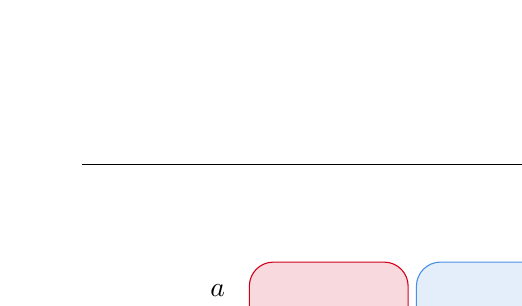
\begin{tikzpicture}[x=0.75pt,y=0.75pt,yscale=-1,xscale=1]
  %uncomment if require: \path (0,163); %set diagram left start at 0, and has height of 163

  %Rounded Rect [id:dp9152961441690106]
  \draw  [color={rgb, 255:red, 208; green, 2; blue, 27 }  ,draw opacity=1 ][fill={rgb, 255:red, 208; green, 2; blue, 27 }  ,fill opacity=0.15 ] (81,33.6) .. controls (81,27.19) and (86.19,22) .. (92.6,22) -- (145.9,22) .. controls (152.31,22) and (157.5,27.19) .. (157.5,33.6) -- (157.5,68.4) .. controls (157.5,74.81) and (152.31,80) .. (145.9,80) -- (92.6,80) .. controls (86.19,80) and (81,74.81) .. (81,68.4) -- cycle ;
  %Rounded Rect [id:dp025551523836803147]
  \draw  [color={rgb, 255:red, 208; green, 2; blue, 27 }  ,draw opacity=1 ][fill={rgb, 255:red, 208; green, 2; blue, 27 }  ,fill opacity=0.15 ] (161.5,95.6) .. controls (161.5,89.19) and (166.69,84) .. (173.1,84) -- (226.4,84) .. controls (232.81,84) and (238,89.19) .. (238,95.6) -- (238,130.4) .. controls (238,136.81) and (232.81,142) .. (226.4,142) -- (173.1,142) .. controls (166.69,142) and (161.5,136.81) .. (161.5,130.4) -- cycle ;
  %Rounded Rect [id:dp5686630594023176]
  \draw  [color={rgb, 255:red, 74; green, 144; blue, 226 }  ,draw opacity=1 ][fill={rgb, 255:red, 74; green, 144; blue, 226 }  ,fill opacity=0.15 ] (161.5,33.6) .. controls (161.5,27.19) and (166.69,22) .. (173.1,22) -- (226.4,22) .. controls (232.81,22) and (238,27.19) .. (238,33.6) -- (238,68.4) .. controls (238,74.81) and (232.81,80) .. (226.4,80) -- (173.1,80) .. controls (166.69,80) and (161.5,74.81) .. (161.5,68.4) -- cycle ;
  %Rounded Rect [id:dp2537296823816999]
  \draw  [color={rgb, 255:red, 74; green, 144; blue, 226 }  ,draw opacity=1 ][fill={rgb, 255:red, 74; green, 144; blue, 226 }  ,fill opacity=0.15 ] (81,95.6) .. controls (81,89.19) and (86.19,84) .. (92.6,84) -- (145.9,84) .. controls (152.31,84) and (157.5,89.19) .. (157.5,95.6) -- (157.5,130.4) .. controls (157.5,136.81) and (152.31,142) .. (145.9,142) -- (92.6,142) .. controls (86.19,142) and (81,136.81) .. (81,130.4) -- cycle ;

  % Text Node
  \draw (14,72.4) node [anchor=north west][inner sep=0.75pt]    {$g_{\mu \nu } =$};
  % Text Node
  \draw (61,31.4) node [anchor=north west][inner sep=0.75pt]    {$a$};
  % Text Node
  \draw (60,57.4) node [anchor=north west][inner sep=0.75pt]    {$b$};
  % Text Node
  \draw (59,92.4) node [anchor=north west][inner sep=0.75pt]    {$\theta $};
  % Text Node
  \draw (60,114.4) node [anchor=north west][inner sep=0.75pt]    {$\phi $};
  % Text Node
  \draw (179,103.4) node [anchor=north west][inner sep=0.75pt]    {$r^{2} d\Omega ^{2}$};


  \end{tikzpicture}
\end{figure}

where we've defined the elements in the red boxes, but the elements in the blue boxes, the cross terms, are still not necessarily zero. We would like to orient our spheres in such a way that all of these cross terms are zero.

Consider a particular point $P$ on sphere $S_P$ and the possible rotations of that sphere. There is a rotation, $R_P$, that leaves $P$ unchanged. Now consider the tangent space $T_P$.There is a subspace of vectors in the tangent space, $T_P$, that rotate into each other under the rotation $R_P$. There is a separate 2-dimensional subspace of $T_P$, that we'll call $V_P$, that remains unchanged (see Figure \ref{fig:rotation}).

\begin{figure}[!h]
  \centering
  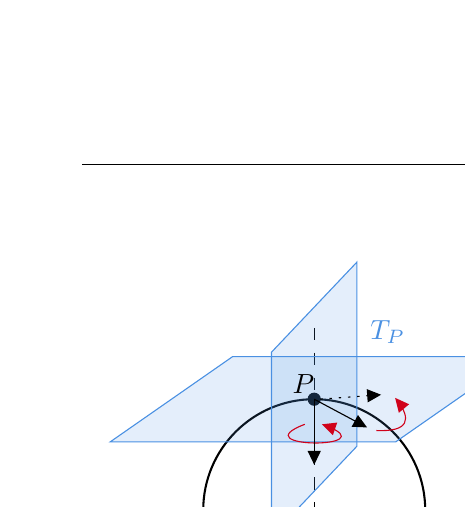
\begin{tikzpicture}[x=0.75pt,y=0.75pt,yscale=-.75,xscale=.75]
  %uncomment if require: \path (0,305); %set diagram left start at 0, and has height of 305

  %Shape: Circle [id:dp22948041466618352]
  \draw  [line width=0.75]  (64.24,164.19) .. controls (64.24,124.8) and (96.16,92.87) .. (135.55,92.87) .. controls (174.93,92.87) and (206.86,124.8) .. (206.86,164.19) .. controls (206.86,203.57) and (174.93,235.5) .. (135.55,235.5) .. controls (96.16,235.5) and (64.24,203.57) .. (64.24,164.19) -- cycle ;
  %Straight Lines [id:da2902359407466264]
  \draw  [dash pattern={on 4.5pt off 4.5pt}]  (135.49,47) -- (135.49,281) ;
  %Curve Lines [id:da30516396490546205]
  \draw [color={rgb, 255:red, 208; green, 2; blue, 27 }  ,draw opacity=1 ]   (129.5,261) .. controls (88.34,276.68) and (182.6,276.99) .. (143.09,261.94) ;
  \draw [shift={(140.5,261)}, rotate = 379.18] [fill={rgb, 255:red, 208; green, 2; blue, 27 }  ,fill opacity=1 ][line width=0.08]  [draw opacity=0] (8.93,-4.29) -- (0,0) -- (8.93,4.29) -- cycle    ;
  %Shape: Circle [id:dp018497056022325875]
  \draw  [fill={rgb, 255:red, 0; green, 0; blue, 0 }  ,fill opacity=1 ] (139.42,92.87) .. controls (139.42,90.73) and (137.69,89) .. (135.55,89) .. controls (133.41,89) and (131.67,90.73) .. (131.67,92.87) .. controls (131.67,95.01) and (133.41,96.75) .. (135.55,96.75) .. controls (137.69,96.75) and (139.42,95.01) .. (139.42,92.87) -- cycle ;
  %Shape: Parallelogram [id:dp45295877051260724]
  \draw  [color={rgb, 255:red, 74; green, 144; blue, 226 }  ,draw opacity=1 ][fill={rgb, 255:red, 74; green, 144; blue, 226 }  ,fill opacity=0.15 ] (83.15,65.5) -- (266.55,65.5) -- (187.95,120.25) -- (4.55,120.25) -- cycle ;
  %Shape: Parallelogram [id:dp9429396510382679]
  \draw  [color={rgb, 255:red, 74; green, 144; blue, 226 }  ,draw opacity=1 ][fill={rgb, 255:red, 74; green, 144; blue, 226 }  ,fill opacity=0.15 ] (108.1,62.68) -- (108.1,180.96) -- (162.99,123.07) -- (162.99,4.79) -- cycle ;
  %Straight Lines [id:da5401896038442613]
  \draw    (135.55,92.87) -- (166.85,109.59) ;
  \draw [shift={(169.5,111)}, rotate = 208.1] [fill={rgb, 255:red, 0; green, 0; blue, 0 }  ][line width=0.08]  [draw opacity=0] (8.93,-4.29) -- (0,0) -- (8.93,4.29) -- cycle    ;
  %Straight Lines [id:da3832167757759517]
  \draw  [dash pattern={on 0.84pt off 2.51pt}]  (139.42,92.87) -- (175.51,90.22) ;
  \draw [shift={(178.5,90)}, rotate = 535.79] [fill={rgb, 255:red, 0; green, 0; blue, 0 }  ][line width=0.08]  [draw opacity=0] (8.93,-4.29) -- (0,0) -- (8.93,4.29) -- cycle    ;
  %Curve Lines [id:da6685921783445326]
  \draw [color={rgb, 255:red, 208; green, 2; blue, 27 }  ,draw opacity=1 ]   (175.5,113) .. controls (197.01,113.94) and (197.53,105.25) .. (189.33,94.31) ;
  \draw [shift={(187.5,92)}, rotate = 410.19] [fill={rgb, 255:red, 208; green, 2; blue, 27 }  ,fill opacity=1 ][line width=0.08]  [draw opacity=0] (8.93,-4.29) -- (0,0) -- (8.93,4.29) -- cycle    ;
  %Curve Lines [id:da11395200374519421]
  \draw [color={rgb, 255:red, 208; green, 2; blue, 27 }  ,draw opacity=1 ]   (129.5,109) .. controls (88.34,124.68) and (182.6,124.99) .. (143.09,109.94) ;
  \draw [shift={(140.5,109)}, rotate = 379.18] [fill={rgb, 255:red, 208; green, 2; blue, 27 }  ,fill opacity=1 ][line width=0.08]  [draw opacity=0] (8.93,-4.29) -- (0,0) -- (8.93,4.29) -- cycle    ;
  %Straight Lines [id:da5767953655887361]
  \draw    (135.55,92.87) -- (135.55,132) ;
  \draw [shift={(135.55,135)}, rotate = 270] [fill={rgb, 255:red, 0; green, 0; blue, 0 }  ][line width=0.08]  [draw opacity=0] (8.93,-4.29) -- (0,0) -- (8.93,4.29) -- cycle    ;

  % Text Node
  \draw (143,276.4) node [anchor=north west][inner sep=0.75pt]  [color={rgb, 255:red, 208; green, 2; blue, 27 }  ,opacity=1 ]  {$R_{P}$};
  % Text Node
  \draw (62,210.4) node [anchor=north west][inner sep=0.75pt]    {$S_{P}$};
  % Text Node
  \draw (120,75.4) node [anchor=north west][inner sep=0.75pt]    {$P$};
  % Text Node
  \draw (170,40.4) node [anchor=north west][inner sep=0.75pt]  [color={rgb, 255:red, 74; green, 144; blue, 226 }  ,opacity=1 ]  {$T_{P}$};

  \end{tikzpicture}
  \caption{The point $P$ is invariant under rotation $R_P$. A vector in $T_P$ is rotated into another vector in $T_P$ and another vector is unchanged.}
  \label{fig:rotation}
\end{figure}

Now consider another point $Q$ on a different sphere that is also invariant under $R_P$. Then there is a geodesic between $P$ and $Q$ that is also unchanged by this rotation (see Figure \ref{fig:geodesic}).

\begin{figure}[!h]
  \centering
  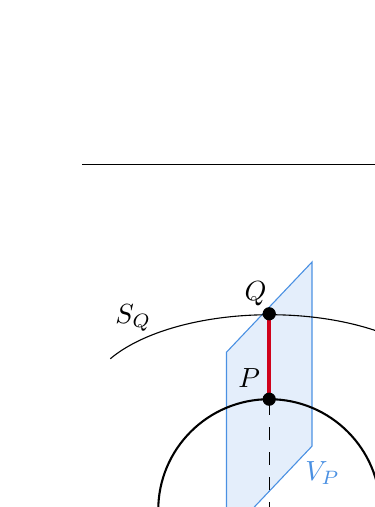
\begin{tikzpicture}[x=0.75pt,y=0.75pt,yscale=-.75,xscale=.75]
  %uncomment if require: \path (0,304); %set diagram left start at 0, and has height of 304

  %Shape: Parallelogram [id:dp2174766573568001]
  \draw  [color={rgb, 255:red, 74; green, 144; blue, 226 }  ,draw opacity=1 ][fill={rgb, 255:red, 74; green, 144; blue, 226 }  ,fill opacity=0.15 ] (90.1,62.68) -- (90.1,180.96) -- (144.99,123.07) -- (144.99,4.79) -- cycle ;
  %Shape: Circle [id:dp8240448416865427]
  \draw  [line width=0.75]  (46.24,164.19) .. controls (46.24,124.8) and (78.16,92.87) .. (117.55,92.87) .. controls (156.93,92.87) and (188.86,124.8) .. (188.86,164.19) .. controls (188.86,203.57) and (156.93,235.5) .. (117.55,235.5) .. controls (78.16,235.5) and (46.24,203.57) .. (46.24,164.19) -- cycle ;
  %Straight Lines [id:da7879500191046807]
  \draw  [dash pattern={on 4.5pt off 4.5pt}]  (117.49,47) -- (117.49,281) ;
  %Curve Lines [id:da5924127758114353]
  \draw [color={rgb, 255:red, 0; green, 0; blue, 0 }  ,draw opacity=1 ]   (111.5,261) .. controls (70.34,276.68) and (164.6,276.99) .. (125.09,261.94) ;
  \draw [shift={(122.5,261)}, rotate = 379.18] [fill={rgb, 255:red, 0; green, 0; blue, 0 }  ,fill opacity=1 ][line width=0.08]  [draw opacity=0] (8.93,-4.29) -- (0,0) -- (8.93,4.29) -- cycle    ;
  %Shape: Arc [id:dp9475099180290631]
  \draw  [draw opacity=0] (15.45,66.9) .. controls (35.28,50.11) and (73.57,38.69) .. (117.55,38.61) .. controls (161.58,38.54) and (199.9,49.85) .. (219.71,66.6) -- (117.55,92.87) -- cycle ; \draw   (15.45,66.9) .. controls (35.28,50.11) and (73.57,38.69) .. (117.55,38.61) .. controls (161.58,38.54) and (199.9,49.85) .. (219.71,66.6) ;
  %Straight Lines [id:da7232564999456332]
  \draw [color={rgb, 255:red, 208; green, 2; blue, 27 }  ,draw opacity=1 ][line width=1.5]    (117.55,38) -- (117.55,92.87) ;
  %Shape: Circle [id:dp5485145642027835]
  \draw  [fill={rgb, 255:red, 0; green, 0; blue, 0 }  ,fill opacity=1 ] (121.42,38) .. controls (121.42,35.86) and (119.69,34.13) .. (117.55,34.13) .. controls (115.41,34.13) and (113.67,35.86) .. (113.67,38) .. controls (113.67,40.14) and (115.41,41.88) .. (117.55,41.88) .. controls (119.69,41.88) and (121.42,40.14) .. (121.42,38) -- cycle ;
  %Shape: Circle [id:dp4001064563381498]
  \draw  [fill={rgb, 255:red, 0; green, 0; blue, 0 }  ,fill opacity=1 ] (121.42,92.87) .. controls (121.42,90.73) and (119.69,89) .. (117.55,89) .. controls (115.41,89) and (113.67,90.73) .. (113.67,92.87) .. controls (113.67,95.01) and (115.41,96.75) .. (117.55,96.75) .. controls (119.69,96.75) and (121.42,95.01) .. (121.42,92.87) -- cycle ;

  % Text Node
  \draw (125,276.4) node [anchor=north west][inner sep=0.75pt]    {$R_{P}$};
  % Text Node
  \draw (44,210.4) node [anchor=north west][inner sep=0.75pt]    {$S_{P}$};
  % Text Node
  \draw (96,71.4) node [anchor=north west][inner sep=0.75pt]    {$P$};
  % Text Node
  \draw (139,131.4) node [anchor=north west][inner sep=0.75pt]  [color={rgb, 255:red, 74; green, 144; blue, 226 }  ,opacity=1 ]  {$V_{P}$};
  % Text Node
  \draw (17,30.4) node [anchor=north west][inner sep=0.75pt]    {$S_{Q}$};
  % Text Node
  \draw (100,15.4) node [anchor=north west][inner sep=0.75pt]    {$Q$};
  \end{tikzpicture}
  \caption{The geodesic between $P$ and $Q$ is tangent to $V_P$ and invariant under $R_P$.}
  \label{fig:geodesic}
\end{figure}

From this we can conclude that there is a set of points in $\mathcal{M}$ that can be reached by geodesics with tangents in $V_P$.

\section{Another visualization}

Another way to visualize this is to draw our sphere with one of the angular coordinates suppressed so that we can see the two coordinates orthogonal to the sphere. Define $O_P$ as the set of points reached by geodesics with tangents in $V_P$. $O_P$ is then invariant under $R_P$.

\begin{figure}[!h]
  \centering
  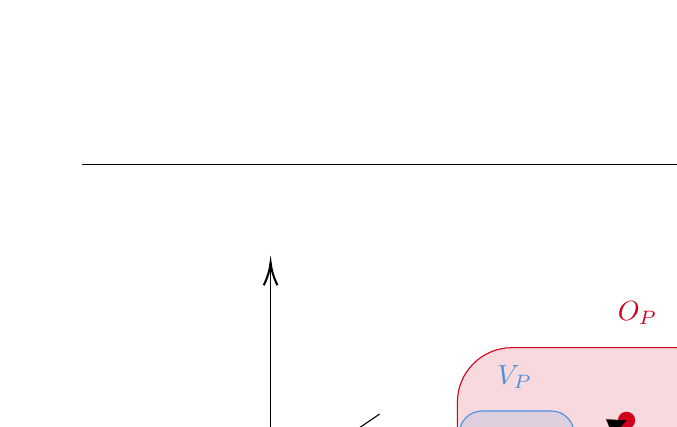
\begin{tikzpicture}[x=0.75pt,y=0.75pt,yscale=-1,xscale=1]
  %uncomment if require: \path (0,187); %set diagram left start at 0, and has height of 187

  %Shape: Circle [id:dp6372095108322378]
  \draw  [color={rgb, 255:red, 208; green, 2; blue, 27 }  ,draw opacity=1 ][fill={rgb, 255:red, 208; green, 2; blue, 27 }  ,fill opacity=1 ] (254.38,79) .. controls (254.38,76.86) and (252.64,75.13) .. (250.5,75.13) .. controls (248.36,75.13) and (246.63,76.86) .. (246.63,79) .. controls (246.63,81.14) and (248.36,82.88) .. (250.5,82.88) .. controls (252.64,82.88) and (254.38,81.14) .. (254.38,79) -- cycle ;
  %Shape: Circle [id:dp4455259589976639]
  \draw  [color={rgb, 255:red, 208; green, 2; blue, 27 }  ,draw opacity=1 ][fill={rgb, 255:red, 208; green, 2; blue, 27 }  ,fill opacity=1 ] (266.38,135) .. controls (266.38,132.86) and (264.64,131.13) .. (262.5,131.13) .. controls (260.36,131.13) and (258.63,132.86) .. (258.63,135) .. controls (258.63,137.14) and (260.36,138.88) .. (262.5,138.88) .. controls (264.64,138.88) and (266.38,137.14) .. (266.38,135) -- cycle ;
  %Shape: Circle [id:dp29553862889868765]
  \draw  [color={rgb, 255:red, 208; green, 2; blue, 27 }  ,draw opacity=1 ][fill={rgb, 255:red, 208; green, 2; blue, 27 }  ,fill opacity=1 ] (218.38,160) .. controls (218.38,157.86) and (216.64,156.13) .. (214.5,156.13) .. controls (212.36,156.13) and (210.63,157.86) .. (210.63,160) .. controls (210.63,162.14) and (212.36,163.88) .. (214.5,163.88) .. controls (216.64,163.88) and (218.38,162.14) .. (218.38,160) -- cycle ;
  %Straight Lines [id:da9801505114841584]
  \draw    (171.25,112) -- (212.49,157.77) ;
  \draw [shift={(214.5,160)}, rotate = 227.98] [fill={rgb, 255:red, 0; green, 0; blue, 0 }  ][line width=0.08]  [draw opacity=0] (8.93,-4.29) -- (0,0) -- (8.93,4.29) -- cycle    ;
  %Rounded Rect [id:dp46014376374894606]
  \draw  [color={rgb, 255:red, 208; green, 2; blue, 27 }  ,draw opacity=1 ][fill={rgb, 255:red, 208; green, 2; blue, 27 }  ,fill opacity=0.15 ] (169,70.3) .. controls (169,55.77) and (180.77,44) .. (195.3,44) -- (274.2,44) .. controls (288.73,44) and (300.5,55.77) .. (300.5,70.3) -- (300.5,154.7) .. controls (300.5,169.23) and (288.73,181) .. (274.2,181) -- (195.3,181) .. controls (180.77,181) and (169,169.23) .. (169,154.7) -- cycle ;
  %Straight Lines [id:da13577106691752405]
  \draw    (79,112) -- (79,5) ;
  \draw [shift={(79,3)}, rotate = 450] [color={rgb, 255:red, 0; green, 0; blue, 0 }  ][line width=0.75]    (10.93,-3.29) .. controls (6.95,-1.4) and (3.31,-0.3) .. (0,0) .. controls (3.31,0.3) and (6.95,1.4) .. (10.93,3.29)   ;
  %Straight Lines [id:da952614181442567]
  \draw    (79,112) -- (197.5,112) ;
  \draw [shift={(199.5,112)}, rotate = 180] [color={rgb, 255:red, 0; green, 0; blue, 0 }  ][line width=0.75]    (10.93,-3.29) .. controls (6.95,-1.4) and (3.31,-0.3) .. (0,0) .. controls (3.31,0.3) and (6.95,1.4) .. (10.93,3.29)   ;
  %Straight Lines [id:da3570195090692969]
  \draw    (131.5,76) -- (3.65,162.88) ;
  \draw [shift={(2,164)}, rotate = 325.8] [color={rgb, 255:red, 0; green, 0; blue, 0 }  ][line width=0.75]    (10.93,-3.29) .. controls (6.95,-1.4) and (3.31,-0.3) .. (0,0) .. controls (3.31,0.3) and (6.95,1.4) .. (10.93,3.29)   ;
  %Shape: Ellipse [id:dp07644752144948863]
  \draw   (108.63,112) .. controls (108.63,102.34) and (122.34,94.5) .. (139.25,94.5) .. controls (156.16,94.5) and (169.88,102.34) .. (169.88,112) .. controls (169.88,121.66) and (156.16,129.5) .. (139.25,129.5) .. controls (122.34,129.5) and (108.63,121.66) .. (108.63,112) -- cycle ;
  %Rounded Rect [id:dp15612920283731446]
  \draw  [color={rgb, 255:red, 74; green, 144; blue, 226 }  ,draw opacity=1 ][fill={rgb, 255:red, 74; green, 144; blue, 226 }  ,fill opacity=0.15 ] (169.88,85.58) .. controls (169.88,79.46) and (174.83,74.5) .. (180.95,74.5) -- (214.18,74.5) .. controls (220.29,74.5) and (225.25,79.46) .. (225.25,85.58) -- (225.25,138.43) .. controls (225.25,144.54) and (220.29,149.5) .. (214.18,149.5) -- (180.95,149.5) .. controls (174.83,149.5) and (169.88,144.54) .. (169.88,138.43) -- cycle ;
  %Straight Lines [id:da05658076062880979]
  \draw    (171.25,112) -- (247.73,80.15) ;
  \draw [shift={(250.5,79)}, rotate = 517.39] [fill={rgb, 255:red, 0; green, 0; blue, 0 }  ][line width=0.08]  [draw opacity=0] (8.93,-4.29) -- (0,0) -- (8.93,4.29) -- cycle    ;
  %Straight Lines [id:da9159989009359304]
  \draw    (171.25,112) -- (259.59,134.27) ;
  \draw [shift={(262.5,135)}, rotate = 194.15] [fill={rgb, 255:red, 0; green, 0; blue, 0 }  ][line width=0.08]  [draw opacity=0] (8.93,-4.29) -- (0,0) -- (8.93,4.29) -- cycle    ;
  %Straight Lines [id:da5166271124498585]
  \draw [color={rgb, 255:red, 74; green, 144; blue, 226 }  ,draw opacity=1 ]   (171.25,112) -- (194.73,102.16) ;
  \draw [shift={(197.5,101)}, rotate = 517.26] [fill={rgb, 255:red, 74; green, 144; blue, 226 }  ,fill opacity=1 ][line width=0.08]  [draw opacity=0] (8.93,-4.29) -- (0,0) -- (8.93,4.29) -- cycle    ;
  %Straight Lines [id:da22239158674567427]
  \draw [color={rgb, 255:red, 74; green, 144; blue, 226 }  ,draw opacity=1 ]   (171.25,112) -- (198.6,119.23) ;
  \draw [shift={(201.5,120)}, rotate = 194.81] [fill={rgb, 255:red, 74; green, 144; blue, 226 }  ,fill opacity=1 ][line width=0.08]  [draw opacity=0] (8.93,-4.29) -- (0,0) -- (8.93,4.29) -- cycle    ;
  %Straight Lines [id:da3058657522959711]
  \draw [color={rgb, 255:red, 74; green, 144; blue, 226 }  ,draw opacity=1 ]   (171.25,112) -- (190.87,133.77) ;
  \draw [shift={(192.88,136)}, rotate = 227.98] [fill={rgb, 255:red, 74; green, 144; blue, 226 }  ,fill opacity=1 ][line width=0.08]  [draw opacity=0] (8.93,-4.29) -- (0,0) -- (8.93,4.29) -- cycle    ;
  %Shape: Circle [id:dp31034792782728604]
  \draw  [fill={rgb, 255:red, 0; green, 0; blue, 0 }  ,fill opacity=1 ] (175.13,112) .. controls (175.13,109.86) and (173.39,108.13) .. (171.25,108.13) .. controls (169.11,108.13) and (167.38,109.86) .. (167.38,112) .. controls (167.38,114.14) and (169.11,115.88) .. (171.25,115.88) .. controls (173.39,115.88) and (175.13,114.14) .. (175.13,112) -- cycle ;
  %Shape: Boxed Bezier Curve [id:dp4209556198846489]
  \draw [color={rgb, 255:red, 0; green, 0; blue, 0 }  ,draw opacity=1 ]   (105.5,109.06) .. controls (93.05,77.79) and (92.74,148.88) .. (104.57,119.89) ;
  \draw [shift={(105.5,117.46)}, rotate = 469.98] [fill={rgb, 255:red, 0; green, 0; blue, 0 }  ,fill opacity=1 ][line width=0.08]  [draw opacity=0] (8.93,-4.29) -- (0,0) -- (8.93,4.29) -- cycle    ;

  % Text Node
  \draw (141.25,132.9) node [anchor=north west][inner sep=0.75pt]    {$S_{P}$};
  % Text Node
  \draw (187,51.4) node [anchor=north west][inner sep=0.75pt]  [color={rgb, 255:red, 74; green, 144; blue, 226 }  ,opacity=1 ]  {$V_{P}$};
  % Text Node
  \draw (173.25,119.28) node [anchor=north west][inner sep=0.75pt]    {$P$};
  % Text Node
  \draw (245,20.4) node [anchor=north west][inner sep=0.75pt]  [color={rgb, 255:red, 208; green, 2; blue, 27 }  ,opacity=1 ]  {$O_{P}$};
  % Text Node
  \draw (80,123.4) node [anchor=north west][inner sep=0.75pt]    {$R_{P}$};


  \end{tikzpicture}
  \caption{With one angular coordinate suppressed, $S_P$ looks like a circle. The blue arrows represent vectors in $V_P$. $O_P$ is the set of points reached by geodesics with tangents in $V_P$.}
  \label{fig:suppressed}
\end{figure}

Figure \ref{fig:q} shows a point $Q$ in $O_P$ and its sphere $S_Q$. This sphere might be at a different time and place.

\begin{figure}[!h]
  \centering
  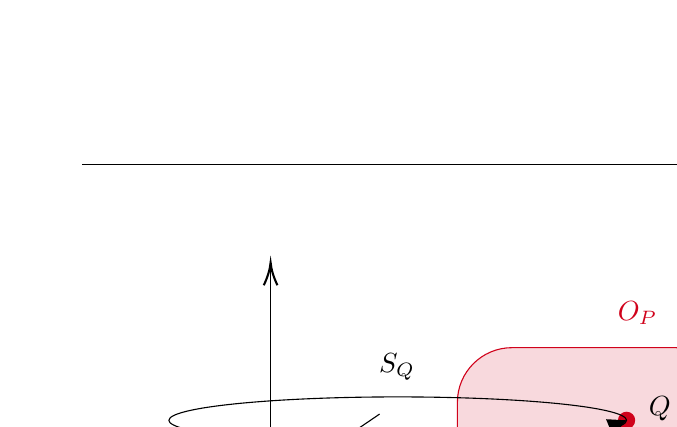
\begin{tikzpicture}[x=0.75pt,y=0.75pt,yscale=-1,xscale=1]
  %uncomment if require: \path (0,187); %set diagram left start at 0, and has height of 187

  %Shape: Circle [id:dp9838488417141364]
  \draw  [color={rgb, 255:red, 208; green, 2; blue, 27 }  ,draw opacity=1 ][fill={rgb, 255:red, 208; green, 2; blue, 27 }  ,fill opacity=1 ] (254.38,79) .. controls (254.38,76.86) and (252.64,75.13) .. (250.5,75.13) .. controls (248.36,75.13) and (246.63,76.86) .. (246.63,79) .. controls (246.63,81.14) and (248.36,82.88) .. (250.5,82.88) .. controls (252.64,82.88) and (254.38,81.14) .. (254.38,79) -- cycle ;
  %Shape: Circle [id:dp5121793793810674]
  \draw  [color={rgb, 255:red, 208; green, 2; blue, 27 }  ,draw opacity=1 ][fill={rgb, 255:red, 208; green, 2; blue, 27 }  ,fill opacity=1 ] (266.38,135) .. controls (266.38,132.86) and (264.64,131.13) .. (262.5,131.13) .. controls (260.36,131.13) and (258.63,132.86) .. (258.63,135) .. controls (258.63,137.14) and (260.36,138.88) .. (262.5,138.88) .. controls (264.64,138.88) and (266.38,137.14) .. (266.38,135) -- cycle ;
  %Shape: Circle [id:dp3036405097098702]
  \draw  [color={rgb, 255:red, 208; green, 2; blue, 27 }  ,draw opacity=1 ][fill={rgb, 255:red, 208; green, 2; blue, 27 }  ,fill opacity=1 ] (218.38,160) .. controls (218.38,157.86) and (216.64,156.13) .. (214.5,156.13) .. controls (212.36,156.13) and (210.63,157.86) .. (210.63,160) .. controls (210.63,162.14) and (212.36,163.88) .. (214.5,163.88) .. controls (216.64,163.88) and (218.38,162.14) .. (218.38,160) -- cycle ;
  %Straight Lines [id:da7600702104223496]
  \draw    (171.25,112) -- (212.49,157.77) ;
  \draw [shift={(214.5,160)}, rotate = 227.98] [fill={rgb, 255:red, 0; green, 0; blue, 0 }  ][line width=0.08]  [draw opacity=0] (8.93,-4.29) -- (0,0) -- (8.93,4.29) -- cycle    ;
  %Rounded Rect [id:dp0011664104615844995]
  \draw  [color={rgb, 255:red, 208; green, 2; blue, 27 }  ,draw opacity=1 ][fill={rgb, 255:red, 208; green, 2; blue, 27 }  ,fill opacity=0.15 ] (169,70.3) .. controls (169,55.77) and (180.77,44) .. (195.3,44) -- (274.2,44) .. controls (288.73,44) and (300.5,55.77) .. (300.5,70.3) -- (300.5,154.7) .. controls (300.5,169.23) and (288.73,181) .. (274.2,181) -- (195.3,181) .. controls (180.77,181) and (169,169.23) .. (169,154.7) -- cycle ;
  %Straight Lines [id:da2222301933142432]
  \draw    (79,112) -- (79,5) ;
  \draw [shift={(79,3)}, rotate = 450] [color={rgb, 255:red, 0; green, 0; blue, 0 }  ][line width=0.75]    (10.93,-3.29) .. controls (6.95,-1.4) and (3.31,-0.3) .. (0,0) .. controls (3.31,0.3) and (6.95,1.4) .. (10.93,3.29)   ;
  %Straight Lines [id:da8846516436041796]
  \draw    (79,112) -- (197.5,112) ;
  \draw [shift={(199.5,112)}, rotate = 180] [color={rgb, 255:red, 0; green, 0; blue, 0 }  ][line width=0.75]    (10.93,-3.29) .. controls (6.95,-1.4) and (3.31,-0.3) .. (0,0) .. controls (3.31,0.3) and (6.95,1.4) .. (10.93,3.29)   ;
  %Straight Lines [id:da5658860552376952]
  \draw    (131.5,76) -- (3.65,162.88) ;
  \draw [shift={(2,164)}, rotate = 325.8] [color={rgb, 255:red, 0; green, 0; blue, 0 }  ][line width=0.75]    (10.93,-3.29) .. controls (6.95,-1.4) and (3.31,-0.3) .. (0,0) .. controls (3.31,0.3) and (6.95,1.4) .. (10.93,3.29)   ;
  %Shape: Ellipse [id:dp45540368845104484]
  \draw   (108.63,112) .. controls (108.63,103.16) and (122.34,96) .. (139.25,96) .. controls (156.16,96) and (169.88,103.16) .. (169.88,112) .. controls (169.88,120.84) and (156.16,128) .. (139.25,128) .. controls (122.34,128) and (108.63,120.84) .. (108.63,112) -- cycle ;
  %Straight Lines [id:da006332923317055261]
  \draw    (171.25,112) -- (247.73,80.15) ;
  \draw [shift={(250.5,79)}, rotate = 517.39] [fill={rgb, 255:red, 0; green, 0; blue, 0 }  ][line width=0.08]  [draw opacity=0] (8.93,-4.29) -- (0,0) -- (8.93,4.29) -- cycle    ;
  %Straight Lines [id:da1990001421085421]
  \draw    (171.25,112) -- (259.59,134.27) ;
  \draw [shift={(262.5,135)}, rotate = 194.15] [fill={rgb, 255:red, 0; green, 0; blue, 0 }  ][line width=0.08]  [draw opacity=0] (8.93,-4.29) -- (0,0) -- (8.93,4.29) -- cycle    ;
  %Shape: Circle [id:dp35887053515914746]
  \draw  [fill={rgb, 255:red, 0; green, 0; blue, 0 }  ,fill opacity=1 ] (175.13,112) .. controls (175.13,109.86) and (173.39,108.13) .. (171.25,108.13) .. controls (169.11,108.13) and (167.38,109.86) .. (167.38,112) .. controls (167.38,114.14) and (169.11,115.88) .. (171.25,115.88) .. controls (173.39,115.88) and (175.13,114.14) .. (175.13,112) -- cycle ;
  %Shape: Boxed Bezier Curve [id:dp8995096291555098]
  \draw [color={rgb, 255:red, 0; green, 0; blue, 0 }  ,draw opacity=1 ]   (105.5,109.06) .. controls (93.05,77.79) and (92.74,148.88) .. (104.57,119.89) ;
  \draw [shift={(105.5,117.46)}, rotate = 469.98] [fill={rgb, 255:red, 0; green, 0; blue, 0 }  ,fill opacity=1 ][line width=0.08]  [draw opacity=0] (8.93,-4.29) -- (0,0) -- (8.93,4.29) -- cycle    ;
  %Shape: Ellipse [id:dp6720903457885754]
  \draw   (30,79) .. controls (30,72.77) and (79.36,67.72) .. (140.25,67.72) .. controls (201.14,67.72) and (250.5,72.77) .. (250.5,79) .. controls (250.5,85.23) and (201.14,90.28) .. (140.25,90.28) .. controls (79.36,90.28) and (30,85.23) .. (30,79) -- cycle ;

  % Text Node
  \draw (141.25,131.4) node [anchor=north west][inner sep=0.75pt]    {$S_{P}$};
  % Text Node
  \draw (173.25,119.28) node [anchor=north west][inner sep=0.75pt]    {$P$};
  % Text Node
  \draw (245,20.4) node [anchor=north west][inner sep=0.75pt]  [color={rgb, 255:red, 208; green, 2; blue, 27 }  ,opacity=1 ]  {$O_{P}$};
  % Text Node
  \draw (80,123.4) node [anchor=north west][inner sep=0.75pt]    {$R_{P}$};
  % Text Node
  \draw (260,66.4) node [anchor=north west][inner sep=0.75pt]    {$Q$};
  % Text Node
  \draw (130,45.4) node [anchor=north west][inner sep=0.75pt]    {$S_{Q}$};
  \end{tikzpicture}
\caption{$S_Q$ might be at a different time or place.}
\label{fig:q}
\end{figure}

Now imagine moving an affine distance $\lambda = 1$ along tangents in $V_p$ to get to each point in $O_P$. We can do this by selecting two independent vectors in $V_P$, $\vv{Y}$ and $\vv{Z}$. Each point in $O_P$ can be reached by $a\vv{Y} + b\vv{Z}$, where $a$ and $b$ are some constants. Note that one of $\vv{Y}$ and $\vv{Z}$ is timelike, and the other is spacelike. We will define $\vv{Y}$ to be the timelike vector.
For some set $a$ and $b$, to get further along in the $a\vv{Y} + b\vv{Z}$ direction (moving the same affine distance $\lambda = 1$), we will need to choose a different $(a,b)$ pair. Define each of these points to have the same $\theta$ and $\phi$ coordinates as $P$: $(\theta_P, \phi_P)$.

\begin{figure}[!h]
  \begin{tikzpicture}[x=0.75pt,y=0.75pt,yscale=-1,xscale=1]
  %uncomment if require: \path (0,140); %set diagram left start at 0, and has height of 140

  %Straight Lines [id:da6192593748390516]
  \draw    (52,70) -- (167.5,26) ;
  \draw [shift={(167.5,26)}, rotate = 339.15] [color={rgb, 255:red, 0; green, 0; blue, 0 }  ][fill={rgb, 255:red, 0; green, 0; blue, 0 }  ][line width=0.75]      (0, 0) circle [x radius= 3.35, y radius= 3.35]   ;
  %Shape: Rectangle [id:dp5094683981364003]
  \draw   (52,13) -- (250.5,13) -- (250.5,127) -- (52,127) -- cycle ;
  %Straight Lines [id:da6301834917384648]
  \draw    (52,70) -- (98.5,70) ;
  \draw [shift={(101.5,70)}, rotate = 180] [fill={rgb, 255:red, 0; green, 0; blue, 0 }  ][line width=0.08]  [draw opacity=0] (8.93,-4.29) -- (0,0) -- (8.93,4.29) -- cycle    ;
  %Straight Lines [id:da9862090033894702]
  \draw    (52,70) -- (52,32) ;
  \draw [shift={(52,29)}, rotate = 450] [fill={rgb, 255:red, 0; green, 0; blue, 0 }  ][line width=0.08]  [draw opacity=0] (8.93,-4.29) -- (0,0) -- (8.93,4.29) -- cycle    ;
  %Shape: Arc [id:dp7671281305617261]
  \draw  [draw opacity=0] (7.03,91.1) .. controls (34.52,85.68) and (51.5,78.23) .. (51.5,70) .. controls (51.5,61.76) and (34.48,54.3) .. (6.93,48.88) -- (-102.25,70) -- cycle ; \draw   (7.03,91.1) .. controls (34.52,85.68) and (51.5,78.23) .. (51.5,70) .. controls (51.5,61.76) and (34.48,54.3) .. (6.93,48.88) ;
  %Shape: Circle [id:dp39506315697356653]
  \draw  [fill={rgb, 255:red, 0; green, 0; blue, 0 }  ,fill opacity=1 ] (55.88,70) .. controls (55.88,67.86) and (54.14,66.13) .. (52,66.13) .. controls (49.86,66.13) and (48.13,67.86) .. (48.13,70) .. controls (48.13,72.14) and (49.86,73.88) .. (52,73.88) .. controls (54.14,73.88) and (55.88,72.14) .. (55.88,70) -- cycle ;
  %Straight Lines [id:da8029712252567158]
  \draw [color={rgb, 255:red, 208; green, 2; blue, 27 }  ,draw opacity=1 ]   (52,70) -- (138.7,37.07) ;
  \draw [shift={(141.5,36)}, rotate = 519.2] [fill={rgb, 255:red, 208; green, 2; blue, 27 }  ,fill opacity=1 ][line width=0.08]  [draw opacity=0] (8.93,-4.29) -- (0,0) -- (8.93,4.29) -- cycle    ;

  % Text Node
  \draw (259,9.4) node [anchor=north west][inner sep=0.75pt]    {$O_{P}$};
  % Text Node
  \draw (78.75,73.4) node [anchor=north west][inner sep=0.75pt]    {$\vec{Z}$};
  % Text Node
  \draw (59,21.4) node [anchor=north west][inner sep=0.75pt]    {$\vec{Y}$};
  % Text Node
  \draw (33,62.4) node [anchor=north west][inner sep=0.75pt]    {$P$};
  % Text Node
  \draw (175.5,17.4) node [anchor=north west][inner sep=0.75pt]    {$( a,b)$};
  % Text Node
  \draw (113.75,46.4) node [anchor=north west][inner sep=0.75pt]  [color={rgb, 255:red, 208; green, 2; blue, 27 }  ,opacity=1 ]  {$a\vec{Y} +b\vec{Z}$};


  \end{tikzpicture}
  \caption{Assigning coordinates $(a,b)$ to each point in $O_P$. Each of these points has angular coordinates $(\theta_P,\phi_P)$.}
  \label{fig:newcoord}
\end{figure}

We can repeat this process for each fixed $(\theta, \phi)$ pair on $S_P$.

Notice that $\vv{\partial_\theta}$ is a tangent to a curve described by $x^\mu = (a_0, b_0, \theta, \phi_0)$, and $\vv{\partial_a}$ is tangent to a curve $x^\mu = (a, b_0, \theta_0, \phi_0)$.
This means that $\vv{\partial_\theta} \cdot \vv{\partial_a} = 0$, so $\vec{g}(\vv{\partial_\theta}, \vv{\partial_a}) = g_{a\theta} = 0$.
Equivalently, $\vv{\partial_\theta} = \tensor{\delta}{_\theta^\mu} \vv{\partial_\mu}$ and $\vv{\partial_a} = \tensor{\delta}{_a^\mu} \vv{\partial_\mu}$.
Therefore, $g_{\mu\nu} \tensor{\delta}{_a^\mu} \tensor{\delta}{_\theta^\nu} = g_{a\theta} = 0$

Similarly,
\[ g_{a\theta} = g_{a\phi} = g_{b\theta} = g_{b\phi} = 0 \]

So we have successfully set the cross terms (in blue) of the metric to zero!

\begin{figure}[!h]
  \centering
  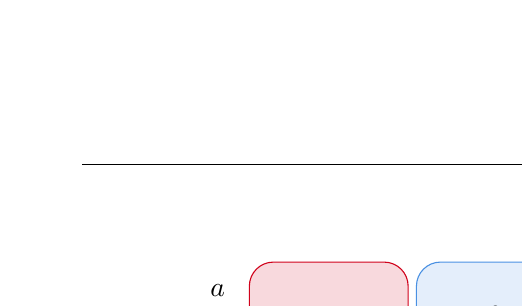
\begin{tikzpicture}[x=0.75pt,y=0.75pt,yscale=-1,xscale=1]
  %uncomment if require: \path (0,163); %set diagram left start at 0, and has height of 163

  %Rounded Rect [id:dp3402002127095296]
  \draw  [color={rgb, 255:red, 208; green, 2; blue, 27 }  ,draw opacity=1 ][fill={rgb, 255:red, 208; green, 2; blue, 27 }  ,fill opacity=0.15 ] (81,33.6) .. controls (81,27.19) and (86.19,22) .. (92.6,22) -- (145.9,22) .. controls (152.31,22) and (157.5,27.19) .. (157.5,33.6) -- (157.5,68.4) .. controls (157.5,74.81) and (152.31,80) .. (145.9,80) -- (92.6,80) .. controls (86.19,80) and (81,74.81) .. (81,68.4) -- cycle ;
  %Rounded Rect [id:dp22852699605929394]
  \draw  [color={rgb, 255:red, 208; green, 2; blue, 27 }  ,draw opacity=1 ][fill={rgb, 255:red, 208; green, 2; blue, 27 }  ,fill opacity=0.15 ] (161.5,95.6) .. controls (161.5,89.19) and (166.69,84) .. (173.1,84) -- (226.4,84) .. controls (232.81,84) and (238,89.19) .. (238,95.6) -- (238,130.4) .. controls (238,136.81) and (232.81,142) .. (226.4,142) -- (173.1,142) .. controls (166.69,142) and (161.5,136.81) .. (161.5,130.4) -- cycle ;
  %Rounded Rect [id:dp08051806364347058]
  \draw  [color={rgb, 255:red, 74; green, 144; blue, 226 }  ,draw opacity=1 ][fill={rgb, 255:red, 74; green, 144; blue, 226 }  ,fill opacity=0.15 ] (161.5,33.6) .. controls (161.5,27.19) and (166.69,22) .. (173.1,22) -- (226.4,22) .. controls (232.81,22) and (238,27.19) .. (238,33.6) -- (238,68.4) .. controls (238,74.81) and (232.81,80) .. (226.4,80) -- (173.1,80) .. controls (166.69,80) and (161.5,74.81) .. (161.5,68.4) -- cycle ;
  %Rounded Rect [id:dp1626107728745949]
  \draw  [color={rgb, 255:red, 74; green, 144; blue, 226 }  ,draw opacity=1 ][fill={rgb, 255:red, 74; green, 144; blue, 226 }  ,fill opacity=0.15 ] (81,95.6) .. controls (81,89.19) and (86.19,84) .. (92.6,84) -- (145.9,84) .. controls (152.31,84) and (157.5,89.19) .. (157.5,95.6) -- (157.5,130.4) .. controls (157.5,136.81) and (152.31,142) .. (145.9,142) -- (92.6,142) .. controls (86.19,142) and (81,136.81) .. (81,130.4) -- cycle ;

  % Text Node
  \draw (14,72.4) node [anchor=north west][inner sep=0.75pt]    {$g_{\mu \nu } =$};
  % Text Node
  \draw (61,31.4) node [anchor=north west][inner sep=0.75pt]    {$a$};
  % Text Node
  \draw (60,57.4) node [anchor=north west][inner sep=0.75pt]    {$b$};
  % Text Node
  \draw (59,92.4) node [anchor=north west][inner sep=0.75pt]    {$\theta $};
  % Text Node
  \draw (60,114.4) node [anchor=north west][inner sep=0.75pt]    {$\phi $};
  % Text Node
  \draw (179,103.4) node [anchor=north west][inner sep=0.75pt]    {$r^{2} d\Omega ^{2}$};
  % Text Node
  \draw (195,42.4) node [anchor=north west][inner sep=0.75pt]    {$0$};
  % Text Node
  \draw (114,103.4) node [anchor=north west][inner sep=0.75pt]    {$0$};
  \end{tikzpicture}
\end{figure}

Now all that's left is to simplify the remaining two blocks (in red).

\section{Simplifying the metric (choosing $a$ and $b$)}

For now, we'll pick the most natural choice: using $r$ as our $b$ coordinate.\sn{This is not always the most useful choice!}
This means that in the $r^2d\Omega^2$ block of the metric, $r^2$ is no longer a function of two coordinates, it's just one of the coordinates, $r$, which we can find by taking the circumference of the sphere and dividing by $2\pi$ (like we did with the Schwarzchild spacetime).
The bottom right block is greatly simplified already!\sn{This relies on the assumption that $\nabla_\mu r \neq 0$, which will be the case for all spacetimes we cover in this class.}

Now we would like to choose a new coordinate $t(a,r)$ that simplifies the remaining block as much as possible. We would like to set
\begin{equation}\label{eq:block1}
  g_{aa}da^2 + 2g_{ar}dadr + g_{rr}dr^2 = fdt^2 + hdr^2
\end{equation}
for some functions $f(t,r)$ and $h(t,r)$ with some clever choice of $t$.

Since $t$ is a function of $a$ and $r$, we can expand $dt^2$ as follows:
\begin{equation}\label{eq:dt2}
   dt^2 = (\partial_a t)^2 da^2 + 2(\partial_a t)(\partial_r t)dadr + (\partial_r t)^2 dr^2
\end{equation}

We can plug Equation \ref{eq:dt2} into Equation \ref{eq:block1} and match the differentials to get the following three equations:
\begin{equation}\label{eq:da2}
  f(\partial_a t)^2 = g_{aa}
\end{equation}
\begin{equation}\label{eq:dadr}
  f(\partial_a t)(\partial_r t) = g_{ar}
\end{equation}
\begin{equation}\label{eq:dr2}
  f(\partial_r t)^2 + h = g_{rr}
\end{equation}

For a known $g_{aa}$, $g_{ar}$, and $g_{rr}$, we now have three equations and three unknowns: $t$, $f$, and $h$.\sn{We will assume that $t(a,r)$ is invertible so that we can write $f$ and $h$ as functions of $a$ and $r$.}
These can, in principle, be solved, and we can use the resulting $t$ as a coordinate. Note that we haven't actually solved for $g_{aa}$, $g_{ar}$, and $g_{rr}$, so we can't solve for $t$ now, but it's possible to do! This reduces the metric down to:\sn{This $f$ is an arbitrary function, \textbf{not} the same as the $f$ we used for the Schwarzchild metric. In fact, if this was the Schwarzchild metric, it would be exactly the negative of the $f$ we used then.}

\begin{equation}\label{eq:finalmetric}
  ds^2 = fdt^2 + hdr^2 + r^2d\Omega^2
\end{equation}

So for a spherically symmetric distribution of matter, we've reduced solving for $g_{\mu\nu}$ down to solving for two unknown functions ($f$ and $h$) of two variables ($t$ and $r$). This may still be very difficult! But we've simplified the problem a lot.

As an aside, something that is often helpful is parameterizing $f$ and $h$ such that they never change signs. In this case, we'll want to assume $f$ is negative definite and $h$ is positive definite:
\begin{equation}\label{eq:f}
  f = -e^{2\alpha(t,r)}
\end{equation}
\begin{equation}\label{eq:h}
  h = e^{2\beta(t,r)}
\end{equation}

These choices are also convenient because we often get derivatives of the metric function divided by the metric function, which cancels out the exponential terms.

Next class, we'll plug these all into Einstein's equations and see what we get!
\end{document}
